\documentclass[]{report}
\usepackage{amsmath}
\usepackage{graphicx}
\usepackage{tabularx}
\usepackage{amsfonts}
\usepackage{amssymb}
\usepackage{amsbsy}

% Title Page
\title{MachineLearning for Visual Computing Aufgabenblock 1}
\author{Christian Br\"andle - Gruppe 5}


\begin{document}
\maketitle

%\begin{abstract}
%\end{abstract}

\chapter{Einfaches Perceptron - Datengeneration}

Gegeben sind vier Datensets a 100 Beobachtungen von 2-dimensionalen Eingangsdaten, welche normalverteilt sind. Die Figuren in Tabelle ~\ref{tab:DataSets} verdeutlichen dies.


\begin{table}[h]
\begin{tabular}{| c | c |}
\hline
 & \\
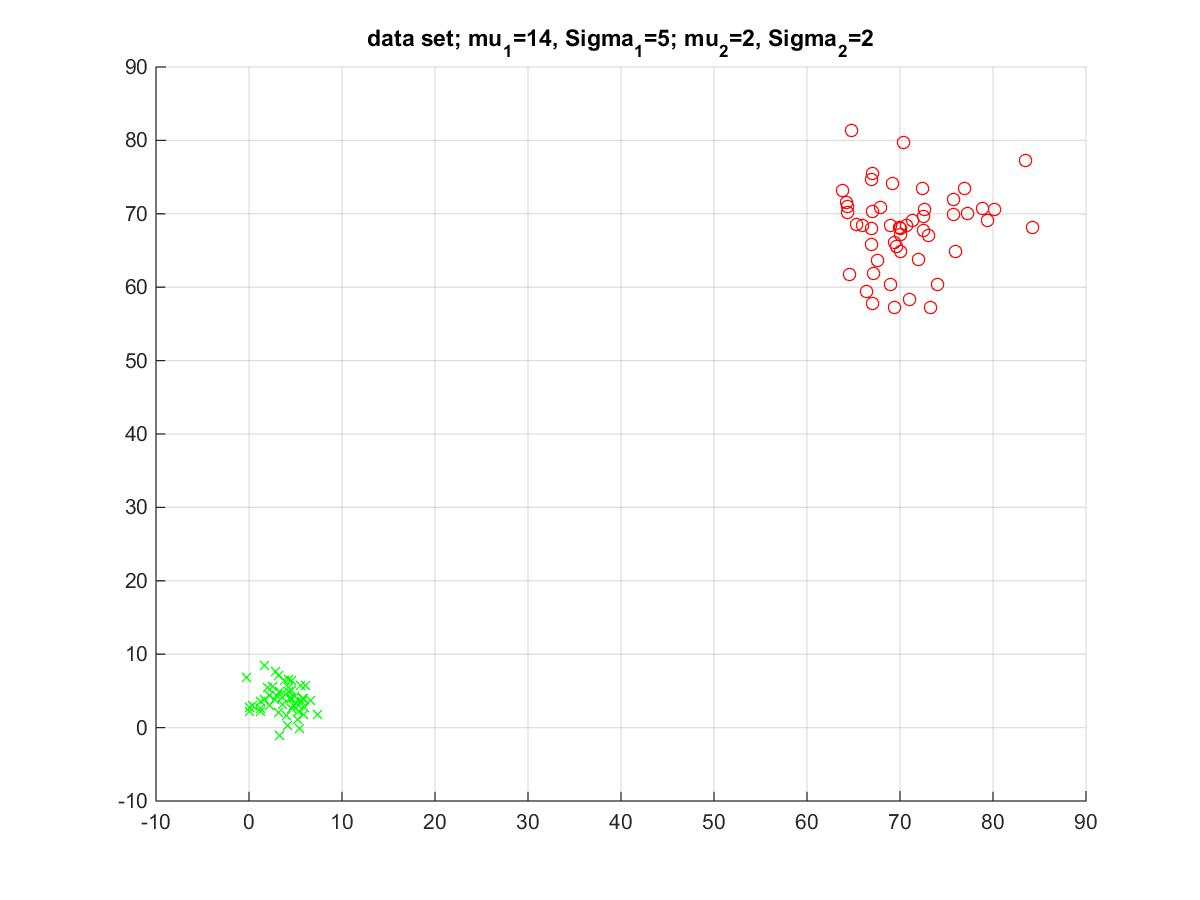
\includegraphics[width=0.4\textwidth]{./images/DataSet_100.jpg} & 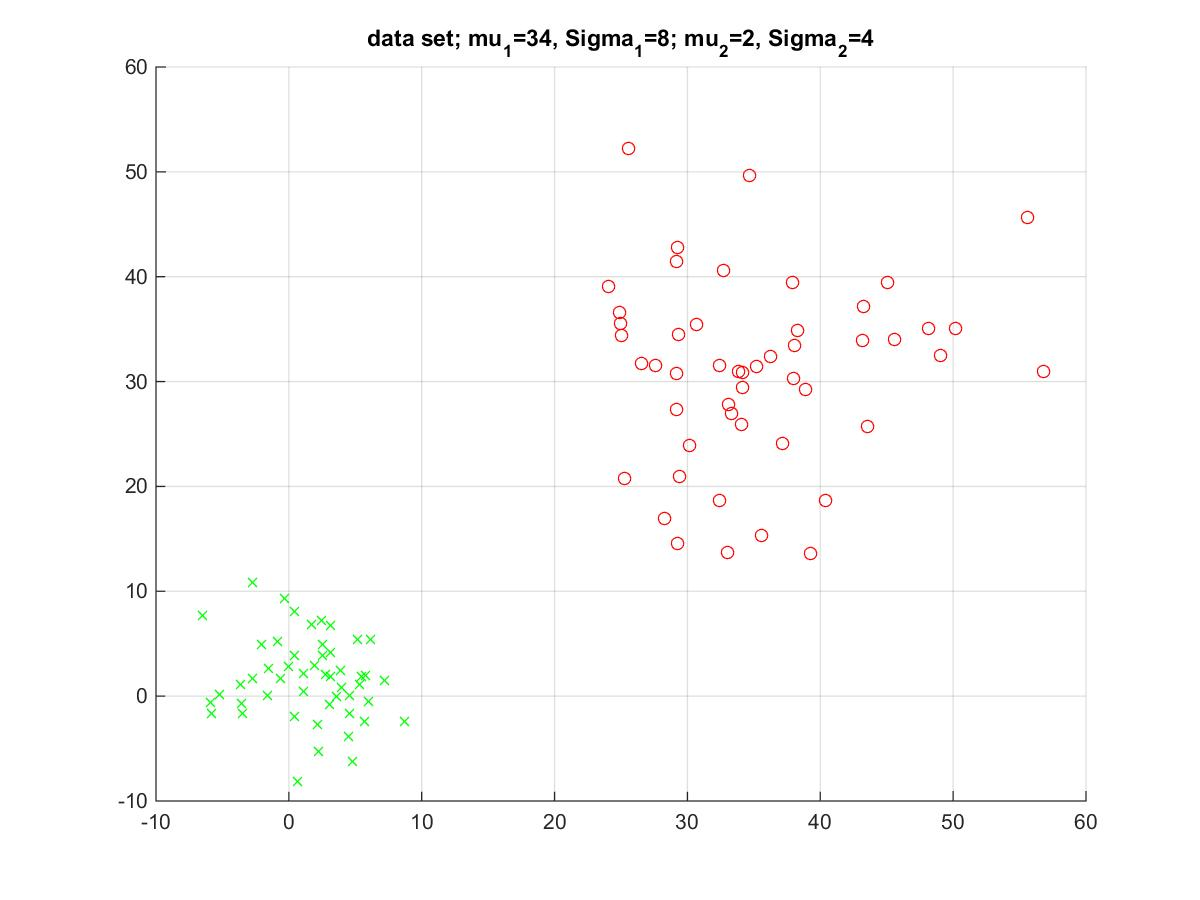
\includegraphics[width=0.4\textwidth]{./images/DataSet_200.jpg} \\
 & \\
 $set_{1}$: $\mu_1=34$, $\Sigma_1=10$ & $set_{1}$: $\mu_1=34$, $\Sigma_1=8$ \\
 $set_{2}$: $\mu_2=2$, $\Sigma_2=2$ & $set_{2}$: $\mu_2=2$, $\Sigma_2=3$ \\
\hline
 & \\
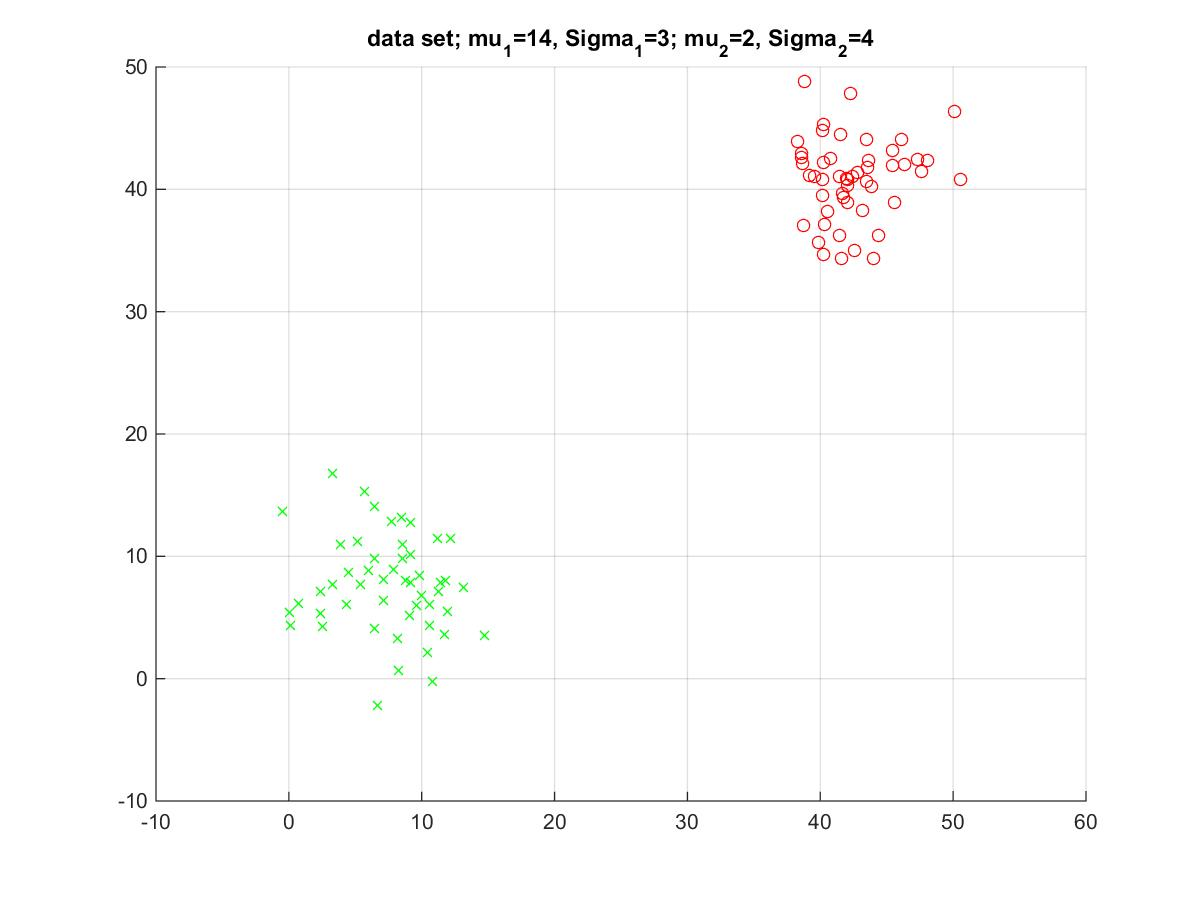
\includegraphics[width=0.4\textwidth]{./images/DataSet_300.jpg} & 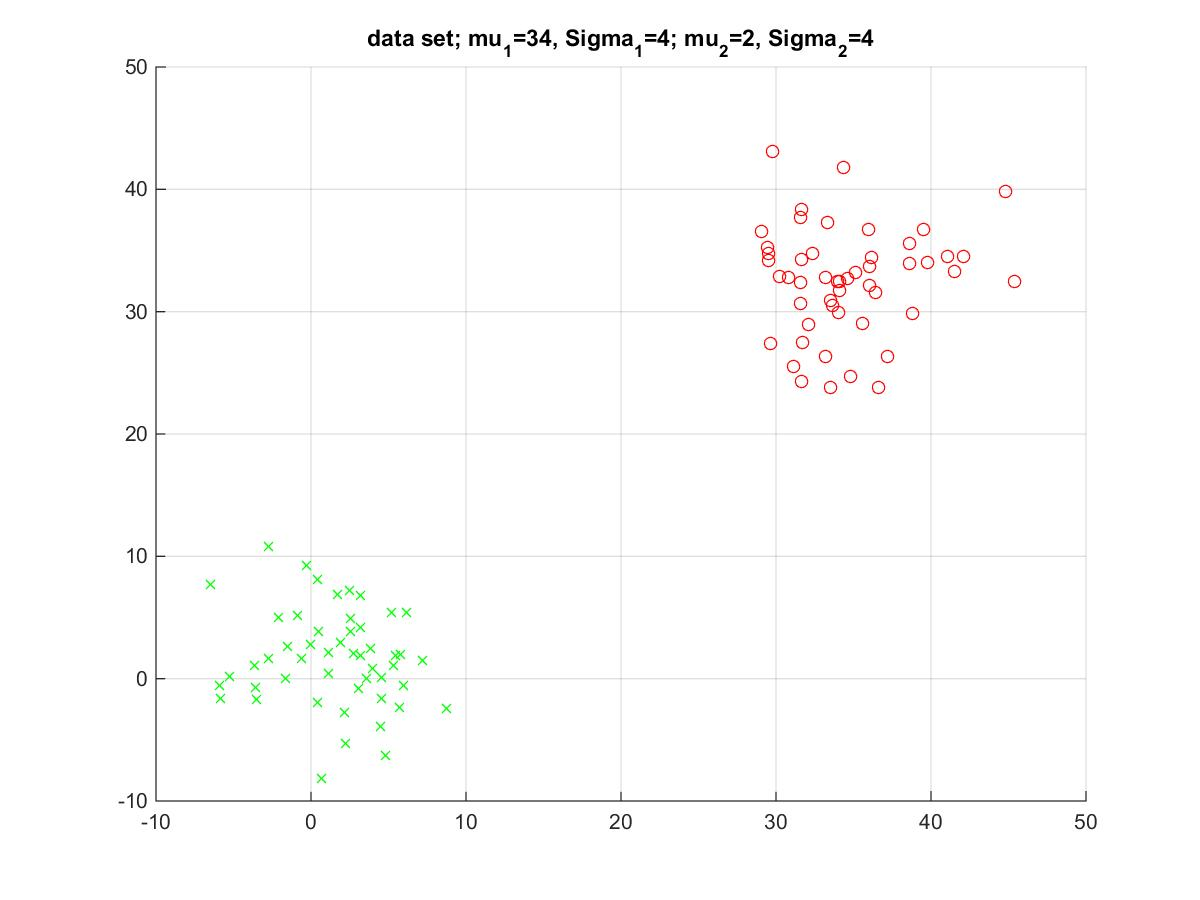
\includegraphics[width=0.4\textwidth]{./images/DataSet_400.jpg} \\
$set_1$: $\mu_1=34$, $\Sigma_1=6$ & $set_1$: $\mu_1=34$, $\Sigma_1=4$ \\
$set_2$: $\mu_2=2$, $\Sigma_2=4$ & $set_2$: $\mu_2=2$, $\Sigma_2=5$ \\
 & \\
\hline
\end{tabular}
\caption{data sets of separatable data}
\label{tab:DataSets}
\end{table}

\section{Einfaches Perceptron - Perceptrontraining}

Im Folgenden wird auf die verschiedenen Trainingsalgorithmen des Perceptrons eingegangen. Die dabei gestellten Fragen nach Geschwindigkeit, Konvergenz und Berechenbarkeit werden in den entsprechenden Punkten behandelt.

\section{Anzahl Iterationen}

Die Anzahl der Iterationen h\"angt ma{\ss}geblich von der \emph{margin} der separierbaren Daten ab. Je kleiner die margin, das hei{\ss}t der Minimalabstand zwischen den beiden Mengen, desto mehr Iterationen sind notwendig, bis der Algorithmus terminiert. Dies ist aus der Angabe der Iterationen aus ~\ref{tab:DataSetsAndBounds} ersichtlich. Weiters ist zu sehen, dass nur der online Perceptron-Trainingsalgorithmus seine Iterationszahl \"andert, die Werte f\"ur den batch Perceptron-Trainingsalgorithmus bleiben konstant.

Bei gr\"o{\ss}eren Datens\"atzen und extrem geringer margin ist ein deutlicher Sprung in der notwendigen Anzahl der Iterationen zu sehen. Exemplarisch wird dies f\"ur die gegebenen vier Datenmengen in Figur ~\ref{fig:meanIterOverDataSets} verdeutlicht.

\begin{figure}[h]
\centering
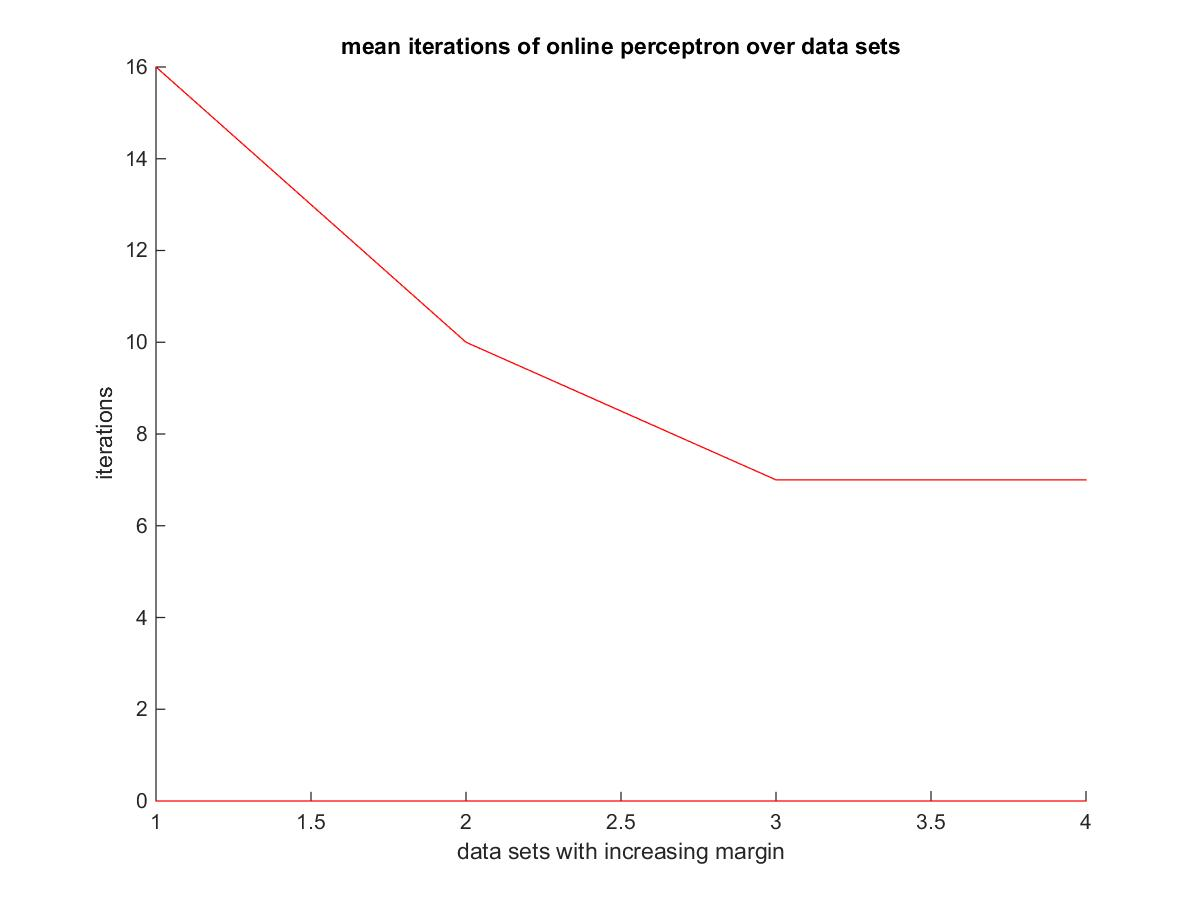
\includegraphics[width=0.4\textwidth]{./images/meanIterOnlinePercOverDataSets.jpg} \\
\caption{iterations of online training for increasing margins}
\label{fig:meanIterOverDataSets}
\end{figure}  

\section{Welchen Einflu{\ss} hat die Schrittweite $\gamma$}

Der Einflu{\ss} der Schrittweite $\gamma$ hat keinerlei Einflu{\ss} auf die Anzahl der notwendigen Iterationen sowohl der online als auch der batch Variante des Perceptron-Trainingsalgorithmus. Die konstante Verteilung der Iterationen \"uber ein $\gamma$ von 0.1 bis 4 f\"ur die jeweiligen unterschiedlichen Datens\"atze in Tabelle ~\ref{tab:GammaToIterations} sowohl f\"ur online als auch batch Variante des Perceptron-Trainingsalgorithmus zu sehen.

\begin{table}[h]
\begin{tabular}{| c | c |}
\hline
 & \\
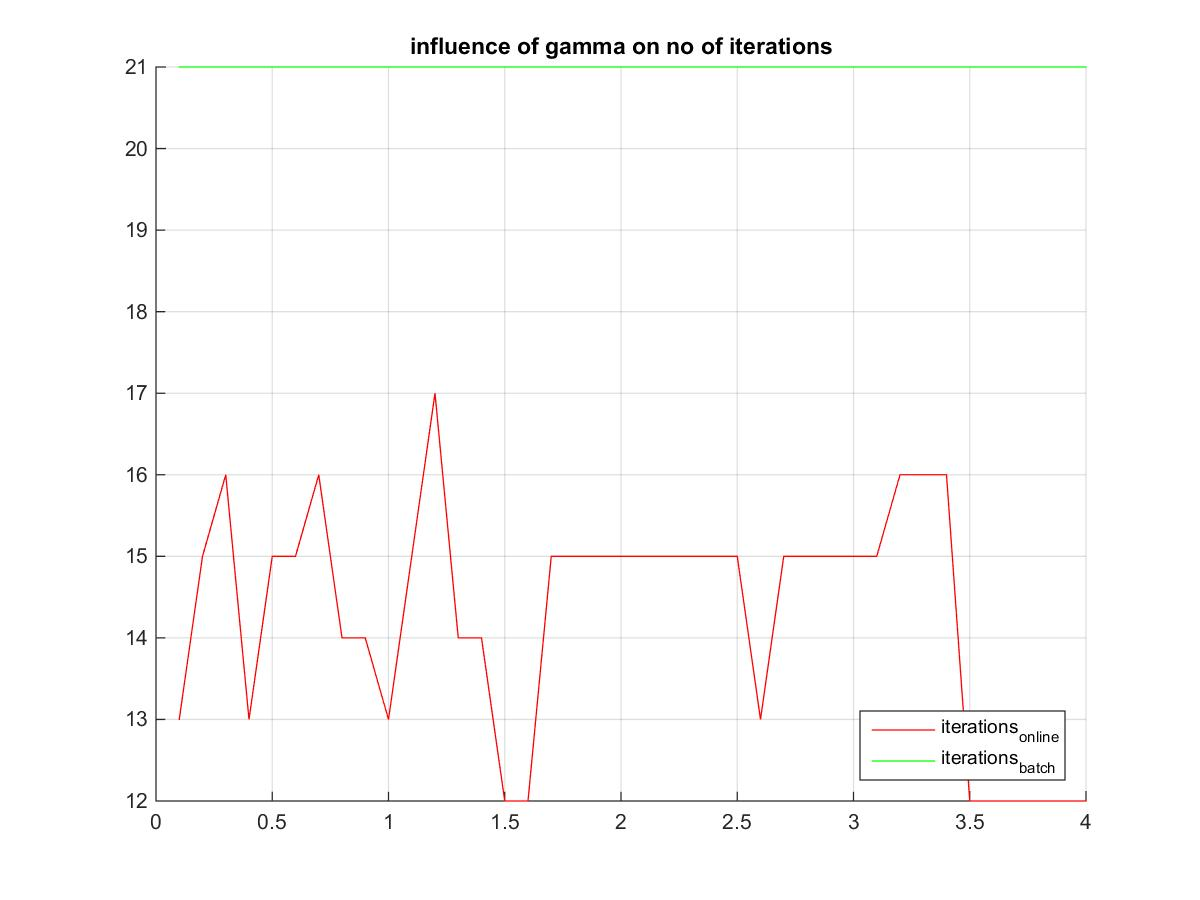
\includegraphics[width=0.4\textwidth]{./images/GammaToIterations_0150.jpg} & 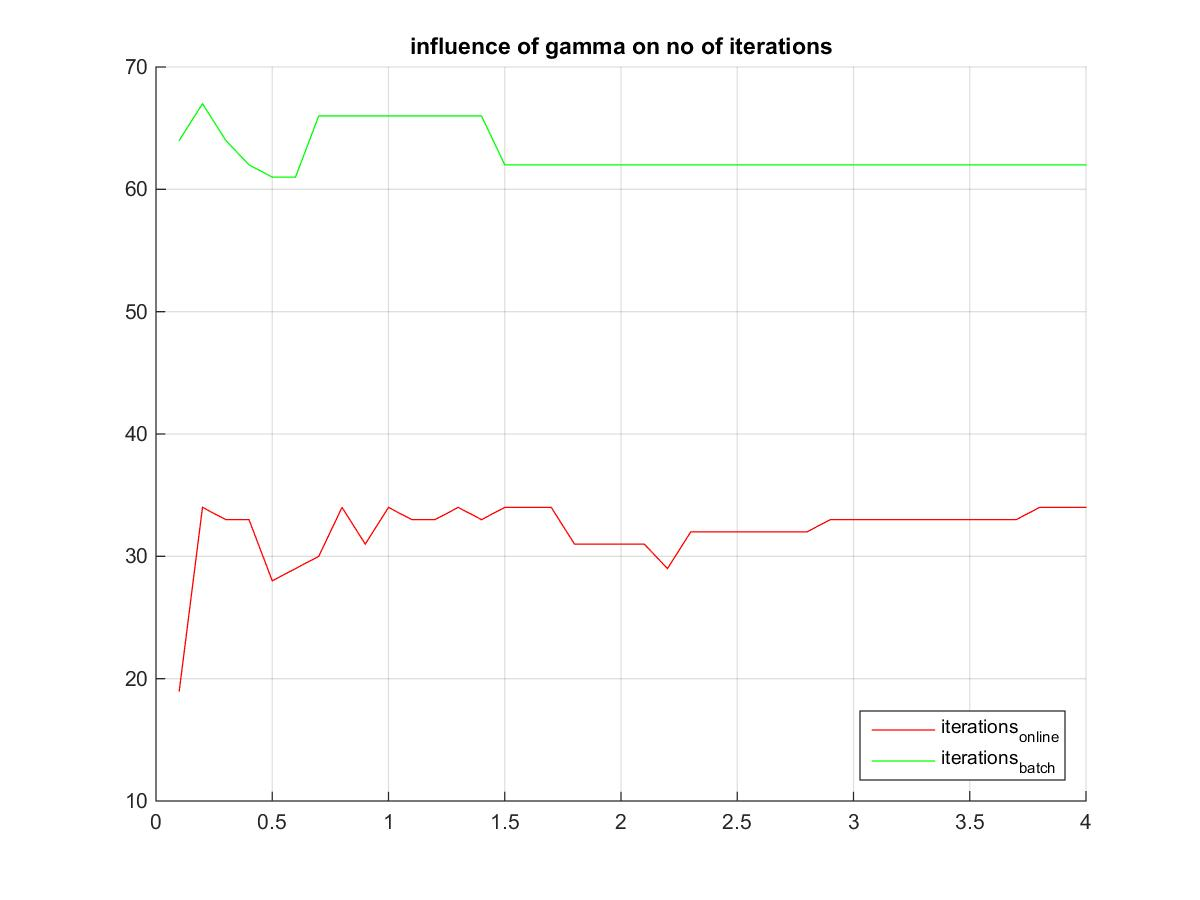
\includegraphics[width=0.4\textwidth]{./images/GammaToIterations_0250.jpg} \\
 & \\
\hline
 & \\
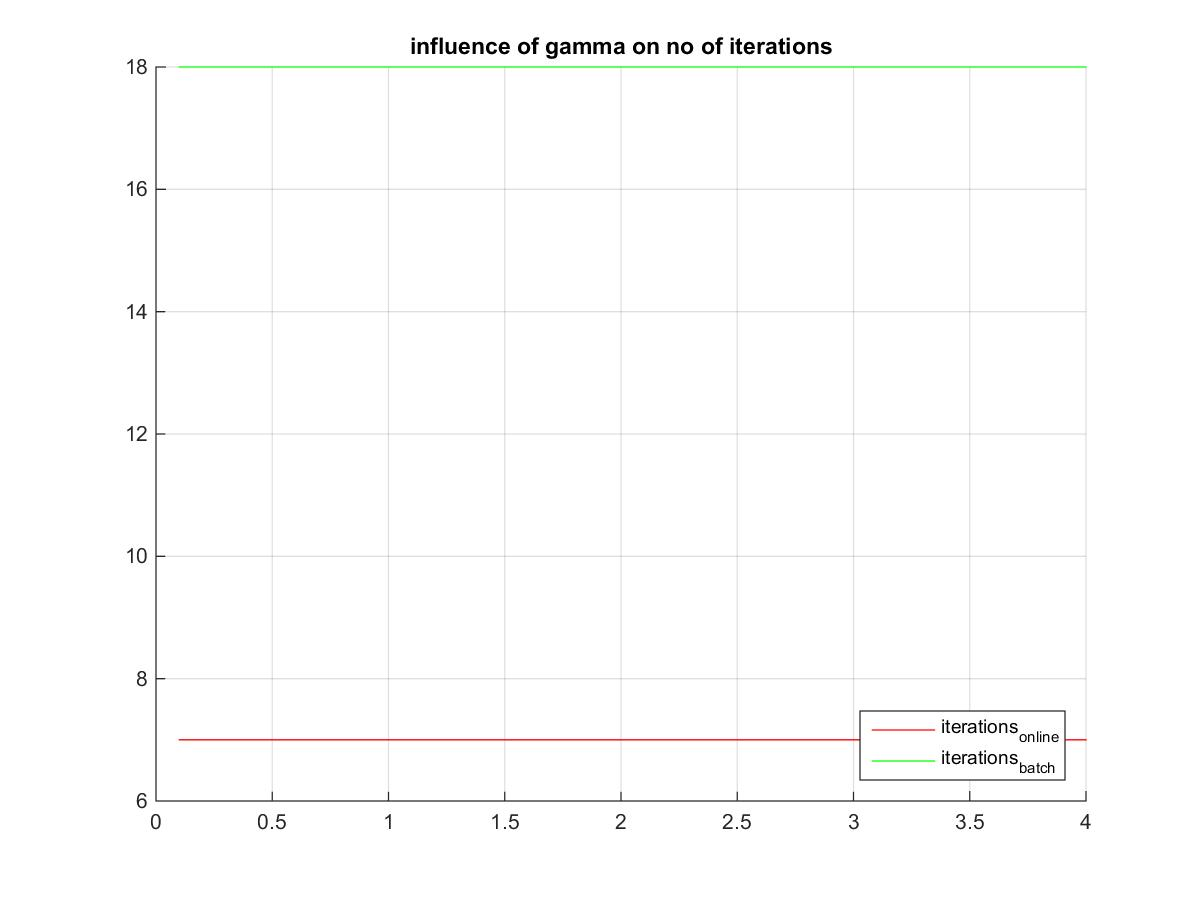
\includegraphics[width=0.4\textwidth]{./images/GammaToIterations_0350.jpg} & 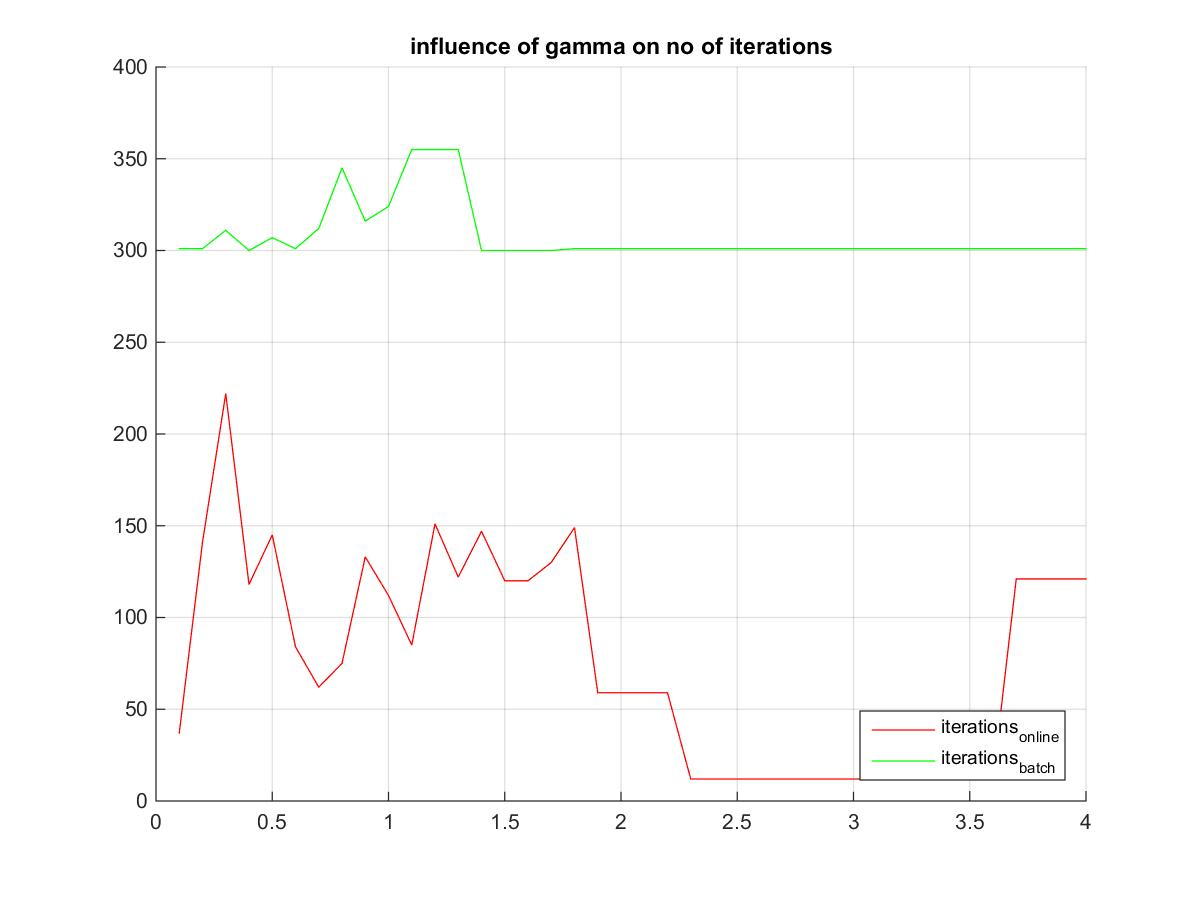
\includegraphics[width=0.4\textwidth]{./images/GammaToIterations_0450.jpg} \\
 & \\
\hline
\end{tabular}
\caption{iteration distribution over gamma}
\label{tab:GammaToIterations}
\end{table}


\section{Daten und Entscheidungsgrenzen im $\mathbb{R}^2$}

Die ermittelten Entscheidungsgrenzen des batch-learning sowie des online-learning Algorithmus sind f\"ur die einzelnen Datens\"atze und ein gegebenes $\gamma=1$ in Tabelle ~\ref{tab:DataSetsAndBounds} zu sehen.

Es ist zu sehen, da{\ss} meistens wesentlich bessere Entscheidungsgrenzen gefunden werden k\"onnten, welche quasi normal auf die margin stehen w\"urden und somit besser noch unbekannte Samples einer korrekten Klasse zuweisen w\"urden.

\begin{table}[h]
\begin{tabular}{| c | c |}
\hline
 & \\
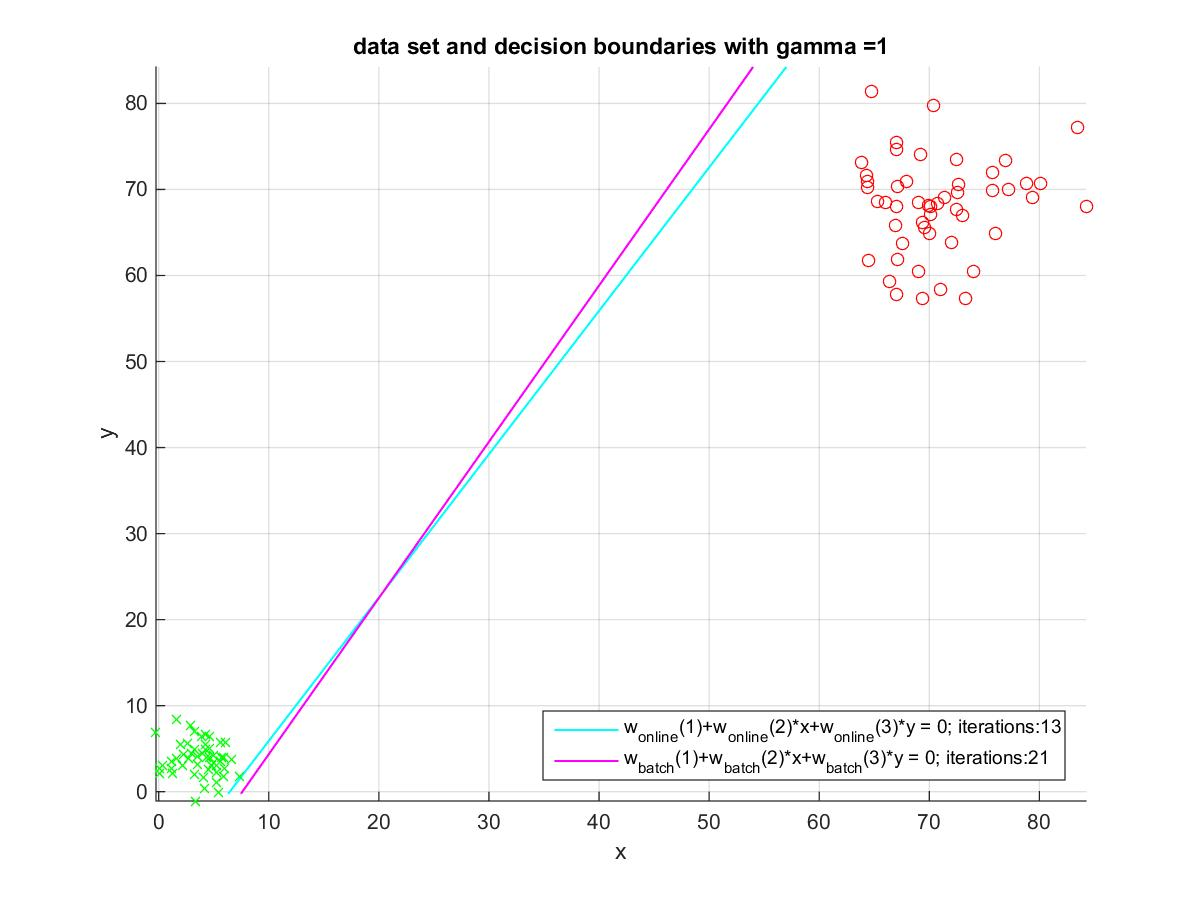
\includegraphics[width=0.4\textwidth]{./images/DataSetAndDecisionBoundary_110.jpg} & 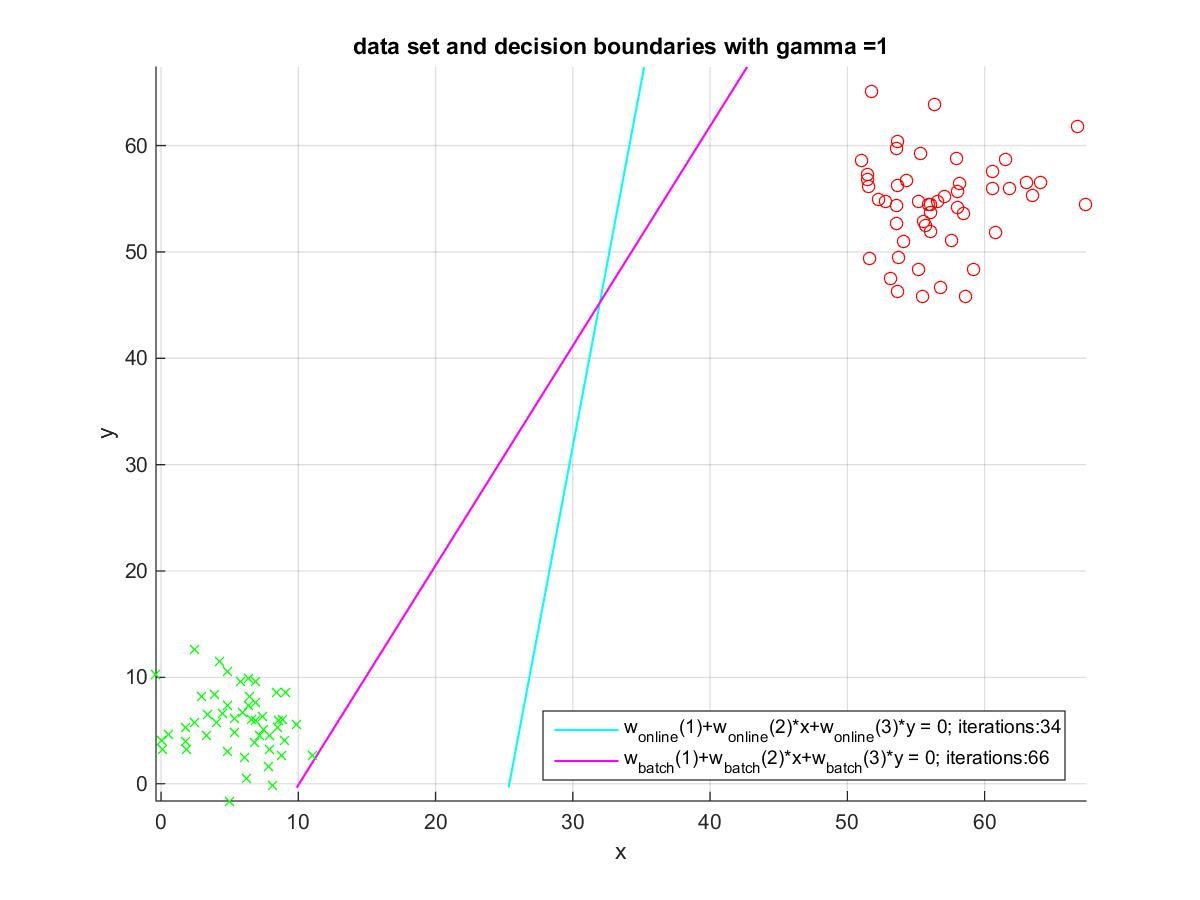
\includegraphics[width=0.4\textwidth]{./images/DataSetAndDecisionBoundary_210.jpg} \\
 & \\
 $set_{1}$: $\mu_1=34$, $\Sigma_1=10$ & $set_{1}$: $\mu_1=34$, $\Sigma_1=8$ \\
 $set_{2}$: $\mu_2=2$, $\Sigma_2=2$ & $set_{2}$: $\mu_2=2$, $\Sigma_2=3$ \\
\hline
 & \\
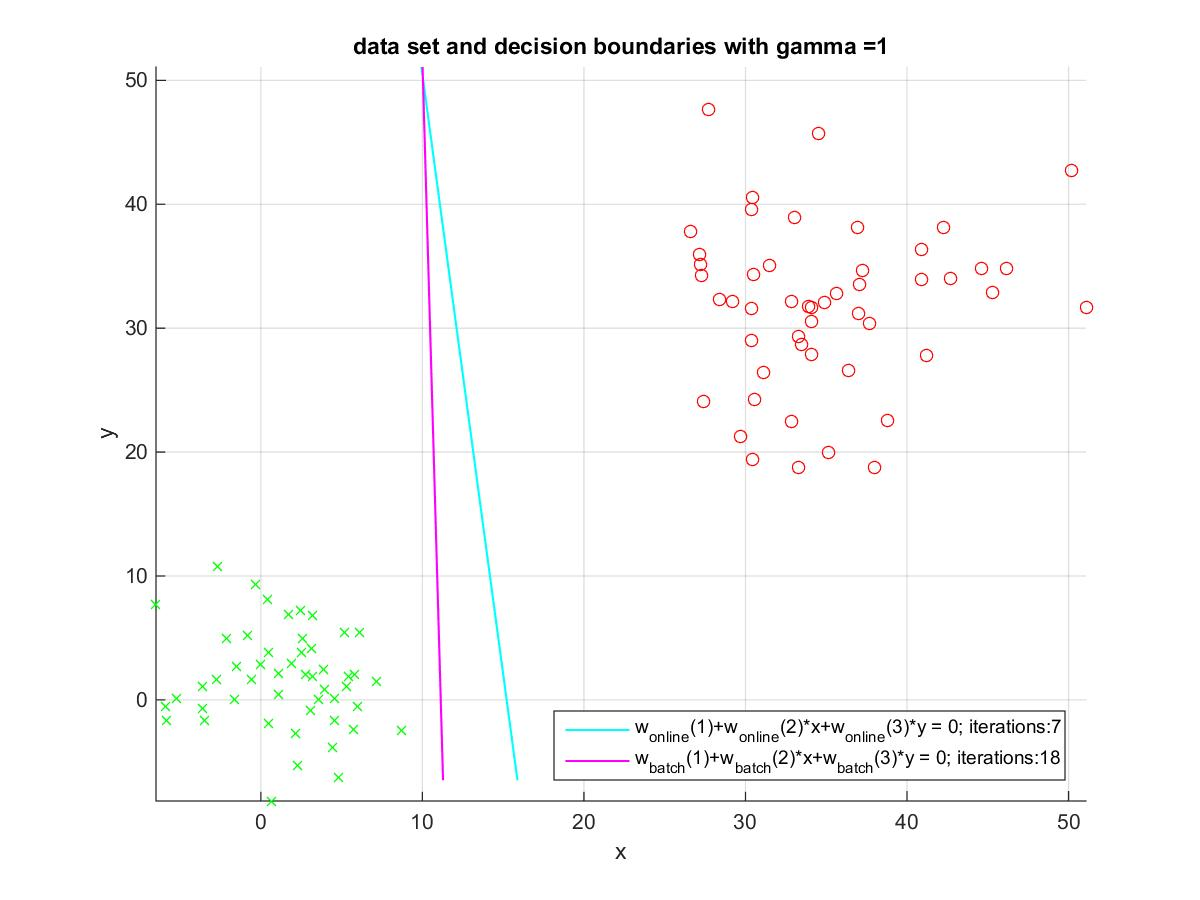
\includegraphics[width=0.4\textwidth]{./images/DataSetAndDecisionBoundary_310.jpg} & 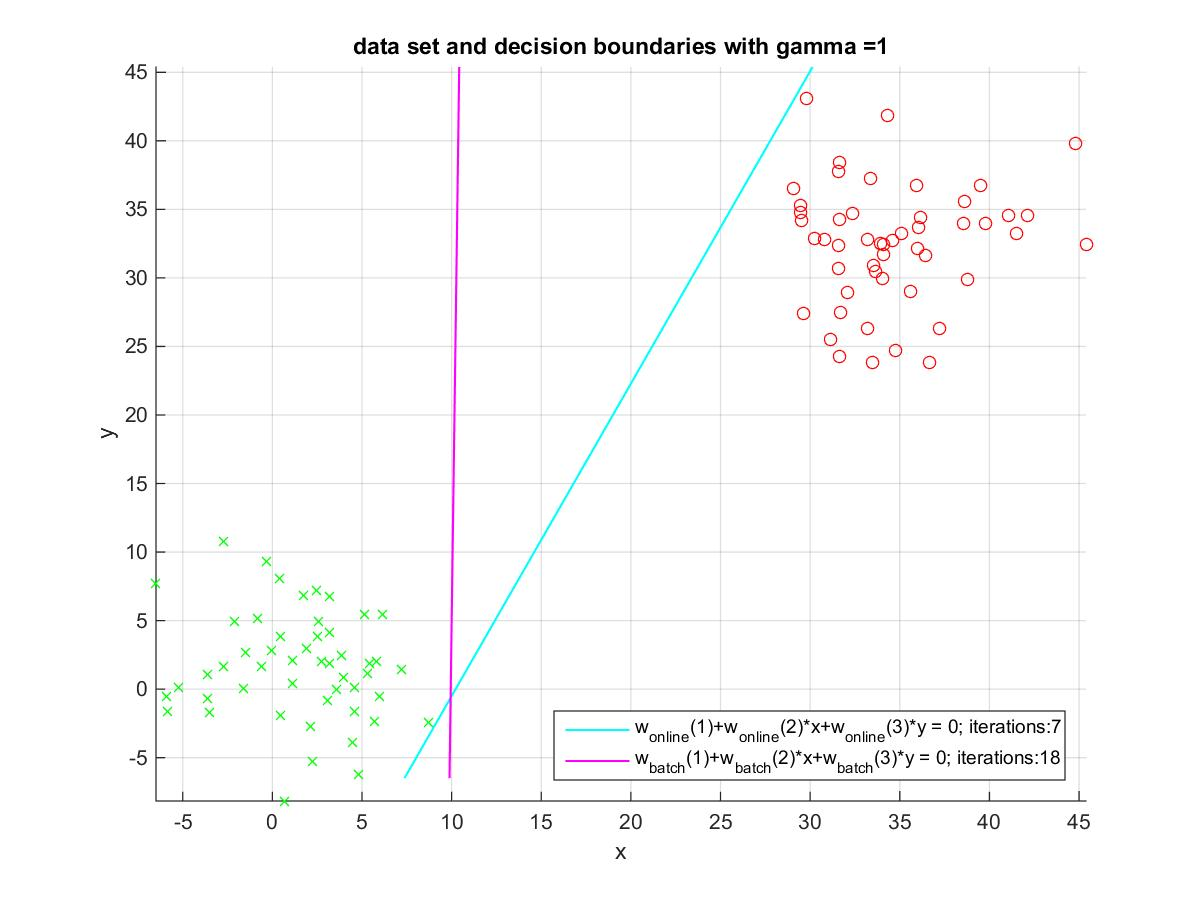
\includegraphics[width=0.4\textwidth]{./images/DataSetAndDecisionBoundary_410.jpg} \\
 & \\
$set_1$: $\mu_1=34$, $\Sigma_1=6$ & $set_1$: $\mu_1=34$, $\Sigma_1=4$ \\
$set_2$: $\mu_2=2$, $\Sigma_2=4$ & $set_2$: $\mu_2=2$, $\Sigma_2=5$ \\
\hline
\end{tabular}
\caption{data sets and decition boundaries}
\label{tab:DataSetsAndBounds}
\end{table}

\section{Wie ist das Verhalten bei nicht linear separierbaren Daten}

Der Algorithmus terminiert nicht da bei jedem Durchlauf Daten gefunden werden, welche in der falschen Klasse landen.

\chapter{Lineare Regression}

Wir erstellen Daten im Bereich von $[0,5]$ mit einer Schrittweite von 0.1 aus der Funkion:

\begin{equation}
y=x^2-Gx+1
\end{equation}

wobei $G=10$ angenommen wird.

Des weiteren erstellen wir eine Trainingsmenge aus jedem sechsten Datenpunkt und f\"ugen je einen Zufallswert aus $N(\mu=0,\Sigma=0.7)$ hinzu.

\section{Gewichtsvektor $w_{online}$ mittels Gradientenabstieg bei quadratischer Fehlerfunktion}

Der Gewichtsvektor $w_{online}$ welcher aufgrund des online Verfahrens f\"ur \emph{LMS} (least mean square) ermittelte wurde kommt in der Anwendung auf die Funktion $f(x)=x^2-Gx+1$ dem optimalen $w^*$ zwar nahe, erreicht dessen Qualit\"at aber nicht. Eine Verringerung der Fehlertoleranz w\"urde hier sicher Abhilfe schaffen.
In der Anwendung auf die Funktion $f(x)$ ergeben sich wie in Figur ~\ref{fig:onlineVsBatchLMS} gezeigt f\"ur die Dimensionalit\"at $3$ die gezeigten Kurven.
  
\begin{figure}[h]
\centering
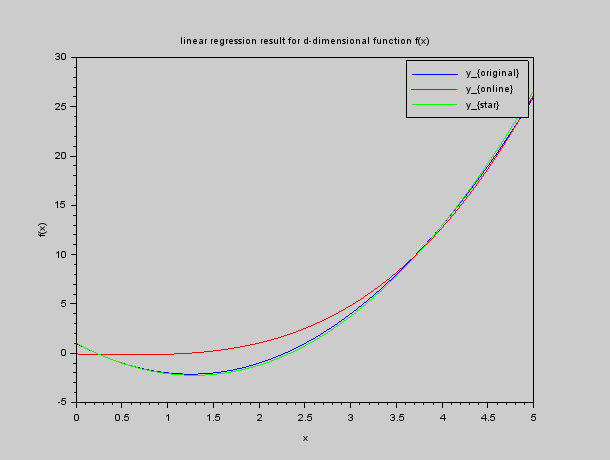
\includegraphics[width=0.4\textwidth]{./images/OnlineVsBatchLMS.png} \\
\caption{online vs batch LMS}
\label{fig:onlineVsBatchLMS}
\end{figure}  

\section{Optimaler Gewichtsvektor $w^*$}

Den optimalen Gewichtsvektor $w^*$ kann man \"uber die Bestimmung der Pseudoinversen $A^+$ f\"ur die Gleichung $Aw^*=b$ ermitteln.
Die Gleichung $w^*=A^+b$ bestimmt das optimale $w^*$. 
Dabei berechnet sich $A^+$ wie folgt:

\begin{eqnarray}
A^+ =& (AA^T)^{-1} &\textnormal{ f\"ur invertierbare } AA^T \\
A^+ =& (AA^T)^{-1} + \lambda I &\textnormal{ f\"ur nicht invertierbare} AA^T \textnormal{ mit } \lambda<<1
\end{eqnarray}

Das ermittelte Ergebnis f\"ur $w^*$ mit normalisierten Daten aus dem $\mathbb{R}^2$ lautet: $w^*=(1.0106678, - 10.0086, 1.8960336, 0.0262634)$.

\section{Konvergenzverhalten in Abh\"angigkeit von Lernrate $\gamma$}

In Figur ~\ref{fig:ConvergenceOverGamma} ist zu sehen, da{\ss} die Anzahl der notwendigen Iterationen um zu einem Optimum zu gelangen mit der Gr\"o{\ss}e von $gamma$ exponentiell abnimmt bis sie bei einem Wert von $\gamma^{hat} \approx 0.0001$ ein Minimum erreichen. Danach steigt die Anzahl der notwendigen Iterationen wieder an.

In Figur ~\ref{fig:ConvergenceOverGammaWDiverge} ist zu sehen, da{\ss} bei Erh\"ohung von $\gamma$ \"uber den optimalen Wert von $\gamma^{hat} \approx 0.0001$ hinaus die Anzahl der Iterationen wieder zunimmt um anschlie{\ss}end einen etwas willk\"urlichen Verlauf anzunehmen. Auf jeden Fall ist festzustellen, dass nach dem erneuten Fallen der Iterationen kein brauchbares Resultat mehr zustande kommt. Exemplarisch wurde dies f\"ur ein $\gamma=0.0035$ durchgerechnet. Eigentlich w\"are erwartet worden, da{\ss} der Algorithmus \"uber einem gewissen $\gamma$ einfach die maximal zul\"assige Anzahl an Iterationen durchf\"uhrt und dann ohne konvergiertes Ergebnis terminiert.

\begin{figure}[h]
\centering
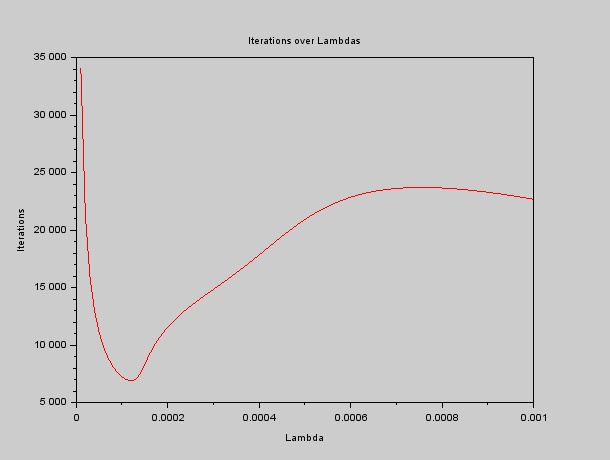
\includegraphics[width=0.4\textwidth]{./images/ConvergenceOverGamma.jpg} \\
\caption{convergence over gamma}
\label{fig:ConvergenceOverGamma}
\end{figure}

\begin{figure}[h]
\centering
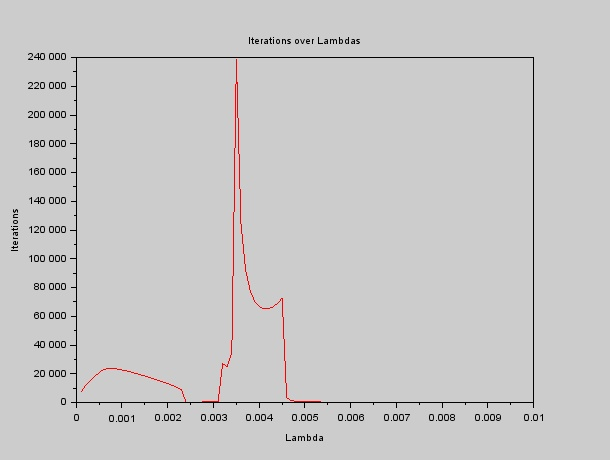
\includegraphics[width=0.4\textwidth]{./images/ConvergenceOverGamma_w_diverge.jpg} \\
\caption{convergence over gamma beyond opmital region}
\label{fig:ConvergenceOverGammaWDiverge}
\end{figure}

\section{Erwartungswert und Varianz von $w^*$ im Bezug zu Dimensionalit\"at $d$ von $f(x)$}

Die Varianz von $w^*$ im Bezug zu Dimensionalit\"at $d$ von $f(x)$ zeigt, da{\ss} je h\"oher die Dimensionalit\"at $d$ steigt, umso h\"oher auch die Varianz $\Sigma$ der ermittelten Werte f\"ur $w^*$ f\"ur verrauschte Eingangsdaten wird. Dies ist auch klar, da h\"oherdimensionale Koeffizienten von $w^*$ h\"ohere Frequenzen repr\"asentieren, welche durch das Verrauschen der Eingangsdaten st\"arker betroffen sind als niedrigere Frequenzen.
Interessanterweise steigt die Varianz aller Koeffizienten von $w^*$ in Tabelle ~\ref{tab:VarianceAndDeviantion} nur bis zu einer Dimensionalit\"at des Problems von $6$, danach f\"allt sie wieder ab. Es ist anzunehmen, dass dies zum Einen aufgrund in Unzul\"anglichkeiten beim generieren der Pseudoinversen zur Berechnung von $w^*$ liegt und zum Anderen in der Tatsache begr\"undet liegt, da{\ss} Frequenzen h\"oherer Ordnung wohl im gegebenen Problem nicht vorkommen.

F\"ur den Mittelwert verh\"alt es sich \"ahnlich. Da das Problem im wesentlichen von der quadratischen Komponente abh\"angt ist diese naturgem\"a{\ss} am deutlichsten vertreten.
H\"oherdimensionale Gewichtsanteile sind nur marginal vertreten.

\begin{table}[h]
\begin{tabular}{| c | c|}
\hline
& \\
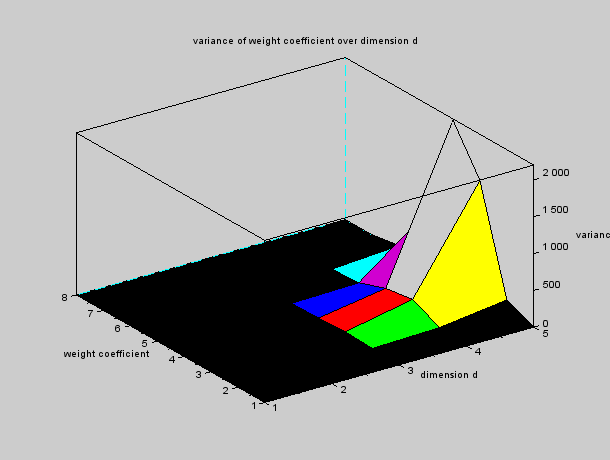
\includegraphics[width=0.4\textwidth]{./images/VarianceWeightCoeffinientsOverDimension_stable.png} & 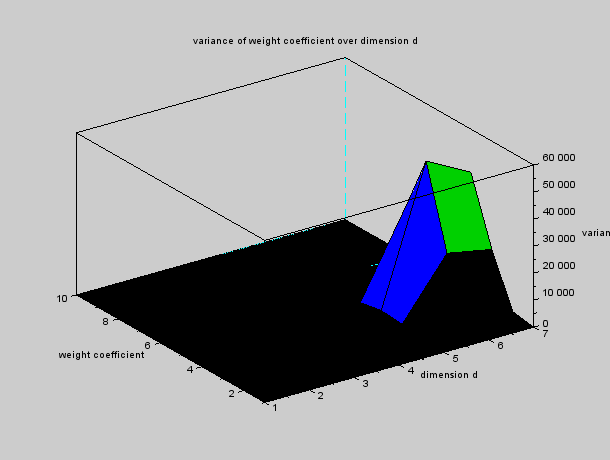
\includegraphics[width=0.4\textwidth]{./images/VarianceWeightCoeffinientsOverDimension.png} \\
variance of weight coefficients & variance of weight coefficients \\
for max. dimension $d=7$ & for max. dimension $d=9$ \\
\hline
\\
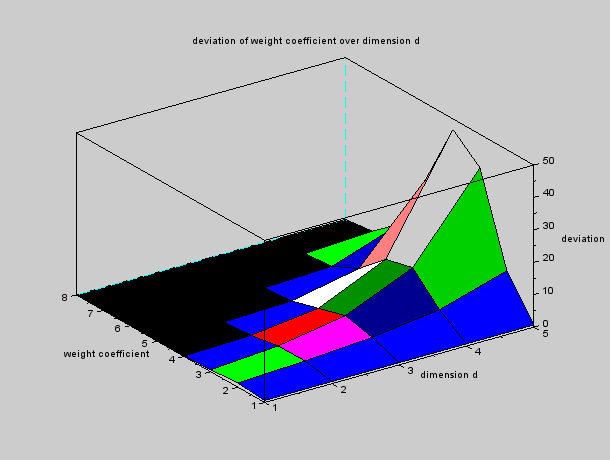
\includegraphics[width=0.4\textwidth]{./images/DeviationWeightCoeffinientsOverDimension_stable.png} & 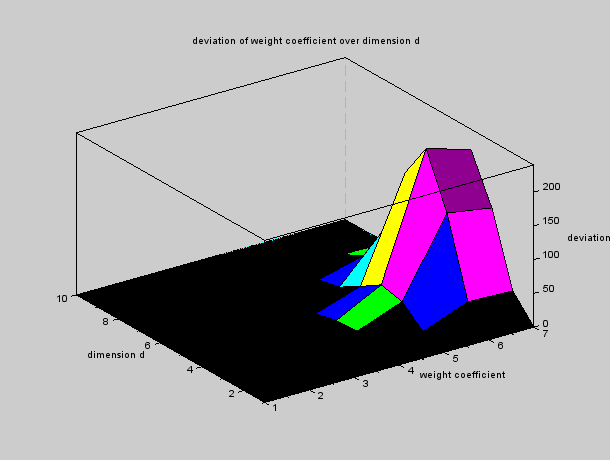
\includegraphics[width=0.4\textwidth]{./images/DeviationWeightCoeffinientsOverDimension.png} \\
deviation of weight coefficients & deviation of weight coefficients \\
for max. dimension $d=7$ & for max. dimension $d=9$ \\
\hline
\\
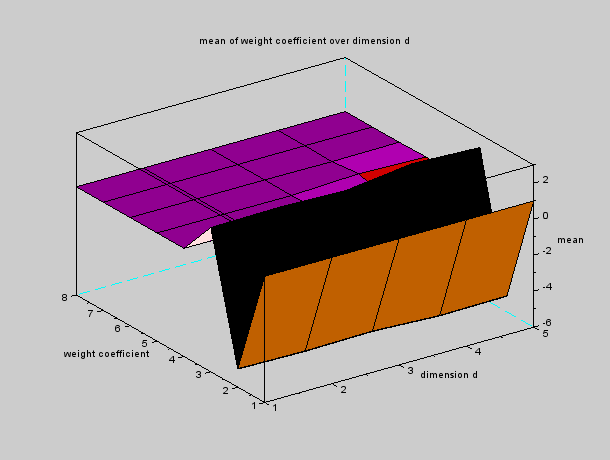
\includegraphics[width=0.4\textwidth]{./images/MeanWeightCoeffinientsOverDimension_stable.png} & 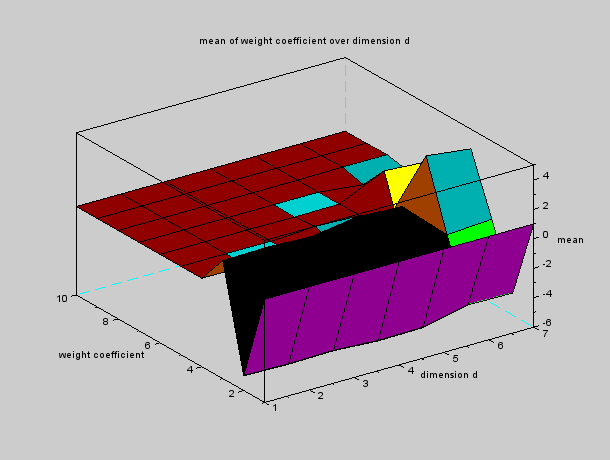
\includegraphics[width=0.4\textwidth]{./images/MeanWeightCoeffinientsOverDimension.png} \\
mean of weight coefficients & mean of weight coefficients \\
for max. dimension $d=7$ & for max. dimension $d=9$ \\
\hline
\end{tabular}
\caption{variance, deviantion and mean of $w^*$ coefficient over dimension}
\label{tab:VarianceAndDeviantion}
\end{table}

Des weiteren ist in Figur ~\ref{fig:Overfitting} festzustellen, dass f\"ur h\"oherdimensionale Gleichungen $f(x)$ basierend auf $w^*$ das overfitting der Kurve $f(x)$ zunimmt, zu sehen in den Schwingungen der Kurven.

\begin{figure}[h]
\centering
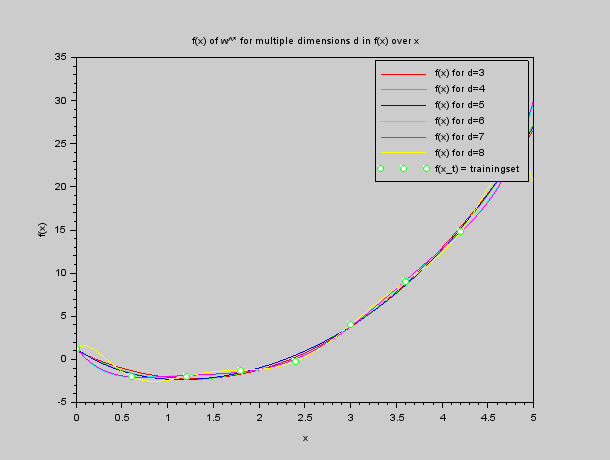
\includegraphics[width=0.4\textwidth]{./images/f_x_w_star_overDimensions_stable.png} \\
\caption{overfitting of $f_{w^*}(x)$ curves over dimension}
\label{fig:Overfitting}
\end{figure}

\section{Mittlere quadratische Abweichung von $f_{w^*}(x^*)$}

Wie erwartet, steigt auch die mittlere quadratische Abweichung von $f_{w^*}(x^*)$ mit der Zunahme der Dimension $d$ an, wie in Figur ~\ref{fig:MeanError} zu sehen ist.

\begin{figure}[h]
\centering
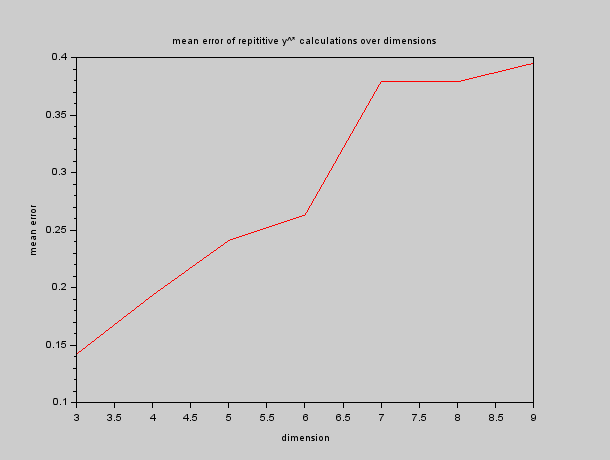
\includegraphics[width=0.4\textwidth]{./images/MeanErrorOverDimensions.png} \\
\caption{mean error of $f_{w^*}(x^*)$ curves over dimension}
\label{fig:MeanError}
\end{figure}

\section{Gewichtsvektor $w^*$ bei ungest\"orter Trainingsmenge \"uber Dimension $d$}

Die resultierenden Kurven f\"ur $f_{w^*}(x)$ welche aus der ungest\"orten Trainingsmenge ermittelt wurden fitten die Originalpunkte aus der Originalkurve $y = 2x^2-Gx+1$ naturgem\"a{\ss} wesentlich besser als die Kurven, welche auf der verrauschen Trainingsmenge basieren. Dies ist in Tabelle ~\ref{tab:f_x_overDimension} zu sehen. Der Ausrei{\ss}er bei Dimension $9$ ist wiederum auf Schw\"achen in der Bestimmung der Pseudoinversen zur\"uckzuf\"uhren.

\begin{table}[h]
\begin{tabular}{| c | c |}
\hline
 & \\
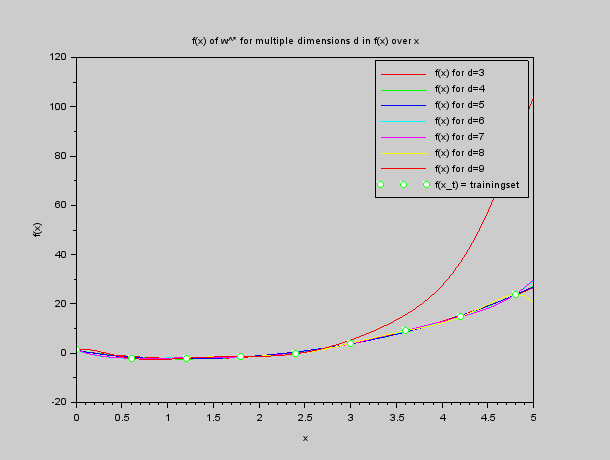
\includegraphics[width=0.4\textwidth]{./images/f_x_w_star_overDimensions.png} & 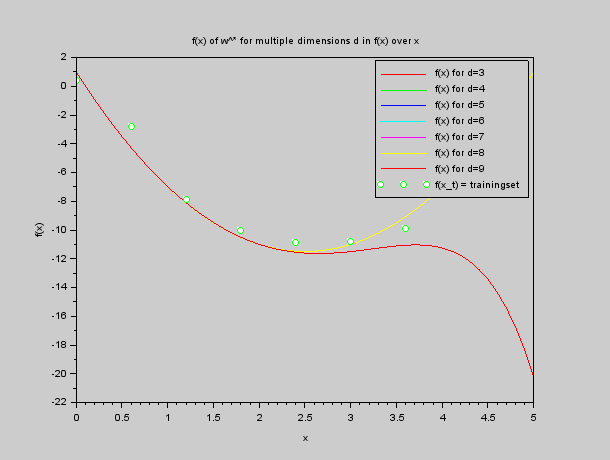
\includegraphics[width=0.4\textwidth]{./images/f_x_w_star_not_preturbed_overDimensions.png} \\
 & \\
 \hline
 & \\
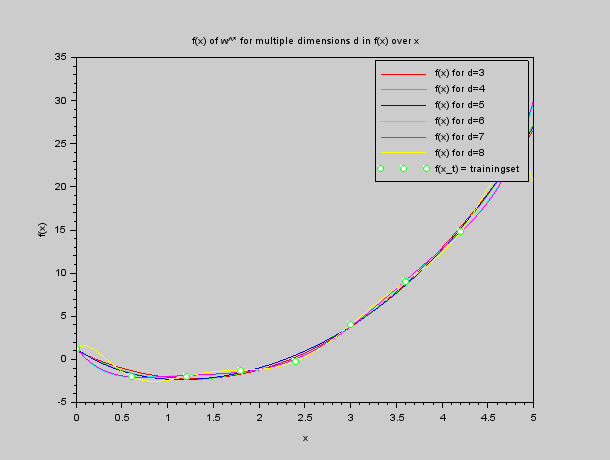
\includegraphics[width=0.4\textwidth]{./images/f_x_w_star_overDimensions_stable.png} & 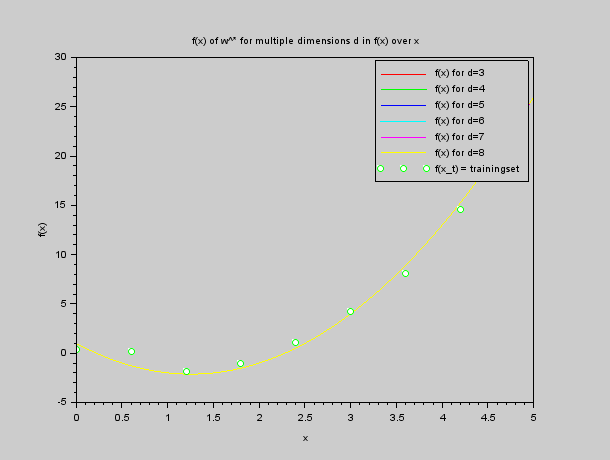
\includegraphics[width=0.4\textwidth]{./images/f_x_w_star_not_preturbed_overDimensions_stable.png} \\
 & \\ 
$w^*$ based on preturbed trainingsset & $w^*$ based on not preturbed trainingsset \\
\hline
\end{tabular}
\caption{$f_{w^*}(x)$ over dimension}
\label{tab:f_x_overDimension}
\end{table}


\end{document}          
